\documentclass[a4paper,openright,11pt]{book}

\newcommand{\ATLASLATEXPATH}{../atlaslatex/latex/}
\usepackage{\ATLASLATEXPATH atlasphysics}
\newcommand{\gmet}{$\gamma +$\met }
\newcommand{\znng}{$\Zboson (\rarrow \nu\nu ) \, + \, \gamma$ }
\newcommand{\zg}{$\Zboson (\rarrow \ell\ell) \,+ \,\gamma$ }
\newcommand{\wg}{$\Wboson (\rarrow \lnu)\, + \, \gamma$ }
\newcommand{\gj}{$\gamma \,  + \,  \text{jets}$ }
\newcommand{\mph}{MonoPhoton }

\usepackage{lettrine}
\usepackage{mparhack}
\usepackage{lipsum}
\usepackage{geometry}
\usepackage{longtable,booktabs,caption}
\usepackage{titlesec}

\usepackage{fancyhdr}
 
\pagestyle{fancy}
\fancyhf{}
\fancyhead[LE]{\itshape \nouppercase  	\rightmark }
\fancyhead[RO]{\itshape \nouppercase \leftmark}
\fancyfoot[LE]{ \thepage}
\fancyfoot[RO]{ \thepage}

\renewcommand{\contentsname}{{Table of Contents}}


\begin{document}
\titleformat{\chapter}[display]{\itshape}{}{2ex}{\fontfamily{ppl}\selectfont\LARGE}[\titlerule]
\frontmatter
\chapter{Introduction}
\lettrine{A}{fter} the discovery of the Higgs boson, many experiment at LHC focused on discovering physics beyond Standard Model. Despite the SM of elementary p articles is a common accepted and well established theory it has many open issue s such the gauge hierarchy problem and {\bfseries other problem introduced in Feng's paper}.
  
  Leading theories proposing to solve this open issues having the common feature of searching for BSM physics are SUSY, large extra dimensions theories and dark matter in the form of weakly interacting massive particles (WIMPs). In other words many attempts are being carried out by theoretical phisicist to find a satisfactory extension of the SM.

  Evidence of new physics might come from missing transverse energy (\MET) in scattering processes. One of the experiment performed by JDM group with the ATLAS detector at LHC is the Mono-Photon Analysis. \MET can of course be trivially associated with neutrinos production but there are other possible explanation to this lack of energy. For instance there are many theories stating that the so-called Dark Matter could be produced in proton proton scattering at the \TeV scale. In this work a new model proposed by M.Cirelli et al. is analyzed. It extends the SM with a EW fermion triplet, which is stable thanks to one of the symmetries already presented in the theory, composed by two charged and one un-charged particles which we assume to be the candidate for DM.

  Since it is a very simple model it is called Minimal Dark Matter model. Unlike other models it has only one parameter from the whole dynamics depends which is the mass of the DM particle.
  
  S  

  Analysing the data collected in 2015 and 2016 with an integrated luminosity of 36.4 \ifb my purpose was to set upper limits on fiducial, but maybe even on the visible, on WIMP production after giving a model independent upper limit on the same physical quantity too. I extimated the main background events that could condition the experiment and reported the outcomes. These events are provided by Monte-Carlo simulation or data-driven techniques normalizing, or fitting, the extimation on data. I took into account both experimental and systematic errors whose contribution is also reported. The techique involved is called ``Trasfer Factor'' techique which provides a parameter $k$ for every Control Region defined which acts as a normalization constant of MC events. 

  No excess of signal are found in the Signal Region and the results are in accordance with the expectation of the SM. 
  Dark Matter candidates are \dots

  Results are interpreted in terms of exclusion limits on fiducial and maybe visible cross section of new phoenomena. Here, you can present te actual results.
  
  Only for illustrative purposes, I'm going to give an overview of what could be found in this thesis. In chapter 1 MDM model is introduced, along with physical motivation of looking for DM. Chapter 2 introduces the LHC facility at CERN and the ATLAS experiment describing the detector and how it works. Fundamentals of MonoPhoton analysis are given in Chapter 4 correlated with a theorical statistical framework. Chapter 5 gets into the heart of the analysis. Here I will report the results for MDM model %4 and 5 potrebbero andare insieme, 5 magari outlook. 1 e 2 potrebbero invertirsi.
  %Darkmatter spiegando la ricerca ai collider e la mono-X+ LHC + MDM con generazione dei campioni fino a validation plots + analysis con bkg fino al limite m.i .

\tableofcontents

\mainmatter
\titleformat{\chapter}[display]{\filcenter\large }{\filcenter\uppercase{Chapter}\thechapter}{2ex}{\bfseries\LARGE\titlerule[1.3pt]\vspace{2ex}\centering}[\vspace{2ex}]
\titleformat{\section}[block]{\filcenter\large }{\thesection}{0pt}{\bfseries	\quad \large \centering}[\vspace{3pt}]
\titleformat{\subsection}[block]{\normalfont \large }{\thesubsection \quad}{0pt}{\itshape \bfseries}[]

\chapter{Fundamentals of the \mph analysis}
Large missing transverse momentum (\met) signature can be sign of evidence of new physics, such as the indirect detection of dark matter.

At LHC we can produce DM particles if they interact with Standard Model particles. A possible candidate to be a constituent of dark matter in universe is given by a weakly interactive mass particle (WIMP) which interacts with SM particles with a strenght similar to the weak interaction so it leaves no track on the detector. Missing transverse momentum can only be measured  if other particles are produced in the collision, for instance a detectable object such jets or photons, in order to tag the WIMP particle production. This kind of analysis are called Mono-X, for one selects events with a single object in final state. In the \mph analysis we are looking for a single high energy photon and large missing transverse momentum signature. The \mph analysis is characterized by a relative clean final state thanks also to a small set of SM processes that produces the same outcome.

For the analysis we are using data collected during 2015 and 2016 with the ATLAS detector, corresponding to an integrated luminosity of $36.4$ \ifb.

In this chapter after describing the software used in the analysis, other than how it performs the fit, and giving a definition of signal and control regions describing the kinematic cuts used to constrain data I present the result for a background only analysis. I report also a brief evaluation of the raise of systematic uncertainties. It conlcudes with some model-independent upper limit results for a discovery analysis.

\section{HistFitter software framework}
\lipsum[1]\marginpar{Qui scrivo qualcosa su HistFitter, come fa il fit.. tipo che costrisce una likelihood che comunque introdutrr\'o pi\'u avanti, che condivide i parametri con tutte le regioni e magari come fa anche il model independent.}

\section{Event selection}
In the context of this \mph analysis several Conotrol Regions (CRs) enriched with the corresponding dominant background in order to extract their normalization on data and a Signal Region (SR) in which eventual signal could be found.

\subsection{Selection in Signal Region}
Events in SR are preselected required by the following property:
\begin{description}%MAGARI CAMBIALO CON UNA DESCRIPTION
\item [Data quality] Data are considered good for physics if belonging to the Good Run List (GRL). They have to be collected in periods in which optimal detector functioning and stable beams were provided;
\item [Trigger acceptance] Events selected must pass the  \verb!HLT_g140_loose! trigger, which {\itshape I think} is a trigger used to detect events with large \met; 
\item [Vertex quality] We take into account events having a primary vertex reconstructed with two associated good-quality tracks with \pt $\ge 400 \,$\MeV and \AetaRange{2.5}
\item [Jet cleaning] Jets tagged with {\itshape BadLoose} (la [38] della nota) in events in which they overlap with photons or leptons with \pt$> 20$ \GeV or not coming from hard scattering are rejected.
\end{description}

After the preselection Candidates in SR are selected with the following kinematic cuts. In order to populate the region with \gmet events, we consider an event to be part of this region if:
\begin{itemize}
\item we compute \met $ \ge 150 $ \GeV;
\item we get one loose photon with \pt $ \ge 150 $ \GeV $\,$ with a pseudorapidity cut in \etaRange{1.52}{2.37} to cut ot the calorimeter crack region and \AetaRange{1.37}
\item \met significance is found to be above $8.5$ \GeV$^{-\frac{1}{2}}$
\item the leading photon is isolated, so that we select events characterized by $ \text{TopoEtcone40} \le 2.45$ \GeV$ + 0.022 \, $\pt \GeV. By this we ensure that in a cone with radius \DeltaRdef $ = 40$, centered in the photon track, all the Topo Clusters have less energy deposited than the one defined above.
\item photon track and \met doesn't overlap, requiring $\Delta\phi_{\gamma - \met} \le 0.4$
\item photon pointing along z coordinate wrt the identified primary vertex must no be larger than $250 \, mm$
\item there is at most one {\itshape good} jet. Even if the analysis is called \mph we take into account events even if they contains a jet, if not we could reject too much statistics as it will be clear in validation plots in section {\bfseries which hasn't been written yet}. Moreover we take only jets such that $\deltaphijetgamma \ge 0.4$

\end{itemize}

In the following section I'm going to deal with all the sources of interference that could affect the SR describing the background processes.

\section{Background estimation}
Alongside the eventual signal coming from unknown ph\oe nomena many other SM processes could pass the cuts defined for the SR ending up being tagged in a wrong way as new physics. We call them background signal, i.e. predictable events that lead to the same signature we are looking for when producing DM particles from \pp scattering.

In other words reasons for events of background can be ascribed to:
\begin{itemize}
\item properly reconstructed SM events which have the same final state as the signal we are looking for;
\item badly reconstructed events in which one (or more) particle are mistaken for photons or they are not reconstructed at all.
\end{itemize}

For the \mph analysis the following background processes were considered.
\begin{itemize}
\item \znng where the two neutrinos produce high \met in the detector. This is the dominant, other than the only irreducible, background as one can see from plots.
\item \wg in which all possible leptonic decay mode of \Wboson are gathered. Here $\ell$ can be an electron being missed or reconstructed as a photon, a muon being missed as well, or a $\tau$ lepton which can decay via hadrons and reconstructed as jet or via leptons and being missed in the detector.
\item \zg where, once again, I am considering all possible leptonic decays for the \Zboson where leptons end up in the same records as in the \Wboson case
\item \gj events in which a jet or photon misreconstruction leads to fake \met.
\item All kind of processes where a jet can fake a photon including:
  \begin{itemize}
  \item double neutrino decay of \Zboson combined with a jet,
  \item leptonic decay of \Wboson along with a jet. If an electron is involved it could fake a photon as well, while we are keeping the jet as pure object for passing SR cuts.
  \end{itemize}
\end{itemize}

In order to quantify the amount of background events in SR, several Control Regions (CRs) are defined which are assumed to be free of signal contamination. Each of them is defined reverting one or more constraints for the SR to enrich every region with a given background process so that they are characterized by a pure dominant process among the others. This provides also ortogonality of a region to one another and their statistical independence.

Events in CRs are simulated via Monte Carlo samples whose prediction must be fitted on data, to get a more reliable estimate of background in SR. This procedure will be explained in detail in section {\bfseries to be written}. A special procedure must be carried out for electron and jets faking photons. In this work results in all the regions for these sources have been taken from previous analysis. However this kind of background cannot be quantified like the previous ones because it is due to some detector mistakes in reconstruction.



\subsection{Transfer factor technique and normalisation of background}
In CRs the respective dominant background can be controlled by comparing MC samples to data. Initial predictions of background in a certain CR must be scaled to observed data in that region, using a normalization factor ($k_{i}$) which is usually computed by a numerical fit by the HistFitter software framework. Usually this procedure is referred as an extrapolation from CRs to SR.

One can define a Trasfer Factor by a mere ratio between MC prediction in SR and MC prediction in a CRs, both unnormalized (raw), and the estimate of the number of events in the signal region for the $i$-th process could be written in terms of event observed in the CRs as:
\begin{equation}
  \label{eqn:TF}
  N_{\textup{est},i}(\text{SR}) =  N_{\textup{obs},i}({\text{CR}}) \times \left[\frac{\text{MC}_{\textup{raw},i}(\text{SR})}{\text{MC}_{\textup{raw},i}(\text{CR})} \right]
\end{equation}

The proper normalization factor is defined as the ratio between events observed and expected in the CRs and equation \ref{eqn:TF} can also be rewritten:
\begin{equation}
  N_{\textup{est},i}(\text{SR}) = k_{i}\times\text{MC}_{\textup{raw},i}(\text{SR})
\end{equation}

By this factor the PDF of every region is rescaled everywhere in the parameter space. Indeed the analysis strategy performed by HistFitter shares the same parameters in all region so that any information found in a single region can be brought to the others.

The advantage of using this procedure is that that systematic uncertainties common to the numerator and the denominator of the TF, such as the uncertainty on luminosity, on the predicted background processes can be canceled at first order in the extrapolation.

\subsection{Definition of Control Regions}
There are four CRs definded in order to extrapolate information on background in Signal Region. In this section a brief definition and differences in kinematic cuts are descrbed.

\begin{description}
\item [One muon CR] In this region one selected muon is requested, kinematic cuts on \pt and \met are the same of those in SR. Here, however, \met is computed in a different way that is the muon energy is added to this variable, so we can treat it as an invisible particle in order to ensure that \met distribution is similar to the one in SR. This region extracts the normalization $k_W$ for \wg background.
\item [Two muon/electron CR] Similarly to the One muon, here we add to \met both muon/electron contribution to \met. Here two selected muons/electrons are required. we can also add a constrain to the invariant mass of the di-lepton to be greater than 20 \GeV\, and less than 1 \TeV \, to avoid any BSM $Z\gamma$ resonances. Moreover we don't require the cut on \met significance. These regions get $k_Z$ for the dominant background \zg in this region which applies via branching ratio to the \znng process.
\item [Photon jet CR] Here kinematic cuts on \met are lowered. We require \met to be in 85 - 110 \GeV\, range to enrich this region of \gj background because in this energy range, probability to have fake \met from jets is higher. To avoid signal contamination we set $\Delta\phi_{\gamma - \met} \le 3.0$ so that we prevent {\itshape back-to-back} signal events to fall in this region. This region, defined in \RunTwo, constrains the normalization for \gj background to get a $k_{pj}$ normalization factor.
\end{description}

{\itshape A priori} a one electron CR could have been defined as well. Nevertheless the one muon CR has enough statistic to constrain the normalization on \Wboson$\gamma$.  This kind of region would have been more difficult to manage even just because electrons could be reconstructed easily as photons which not happens for muons being detected far away in the detector from photons increasing the number of \gj events contamination. In the analysis carried out in [nota di supporto] one evince that no improvement on $k_W$ error can be seen, instead there is a raise of $k_{pj}$ error due to furhter background contamination.

As mentioned earlier fake photons from electrons and jets enter the fit as given values and it is not constrained by any region. They have been estimated via data driven tecniques in other analysis.

\section{Results for a background-only fit}
{\bfseries To be written}

%\chapter[MonteCarlo samples production]{MonteCarlo production of Minimal DM model samples for the \mph analysis}
\label{chapt:mc}

\lettrine{T}{}his chapter describes all the steps made to generate, simulate and reconstruct MonteCarlo (MC) events in the context of the Minimal DM model for the \mph analysis .

%In the \mph analysis, which is a ``cut\&count'' analysis (refer to Chapt. \ref{chapt:mph}), we are looking for a single high energy photon and large missing transverse momentum (\met) signature, whose definition will be given in \Sect{\ref{sec:recoreal}}. Therefore it is characterized by a relative clean final state thanks also to a small set of SM processes that produces the same outcome. The Minimal DM model predicts several ways in which DM can be produced and revealed within a \mph analysis. Three examples of Feynman diagram are given in \Fig{\ref{fig:feynman}}. Notice that a photon can also be radiated from the final state which is a peculiarity with respect to other DM simplified models adopted at LHC.

The simulation of the physics processes in the detector is a fundamental ingredient in the analysis to assess the discovery potential for a new signal but also as input to the real data scrutiny.
%In order to study the detector response for a wide range of physics processes and scenarios, 
A detailed simulation  of the physics process and of the detector response is pursued providing an output format which is identical to that of the true detector. 

The simulation process of events comes across several steps. The first one is the event generation in which the products of \pp collision are simulated. The event generation starts with the creation of the list of particles (electrons, photons, partons\dots) from the hard scattering. The partons radiation is modeled through \emph{parton shower}, finally hadronization and underlying events are also used to complete the event. This step consists in the Truth-level simulation, producing an EVNT file, and a summary file (a TRUTH file) can be built from this events at particle level.

The second step consists in the simulation of how particles interact with the detector which is followed by the digitization of the events. The simulation program is integrated into the ATLAS software framework, Athena, and uses the \geant \cite{geant4} simulation toolkit. Detailed description of the ATLAS Simulation Infrastructure is given in~\cite{simulation}.

Afterwards the simulated event can be passed to the reconstruction software in the same way as actual recorded data. Then all the events reconstructed are filtered by a derivation code which selects only the  relevant events for a specific analysis. Finally the ``derivated'' events are collected in a compact and practical ROOT file, i.e a NTUPLE, ready to be processed by the analysis.

For this analysis the software chain described above, and shown in \Fig{\ref{fig:chain}}, was run in batch mode on the Milano Tier3 computing facility via HTCondor$^{\textup{TM}}$.


\begin{figure}[t]
\centering
{\fontfamily{pag}\selectfont  
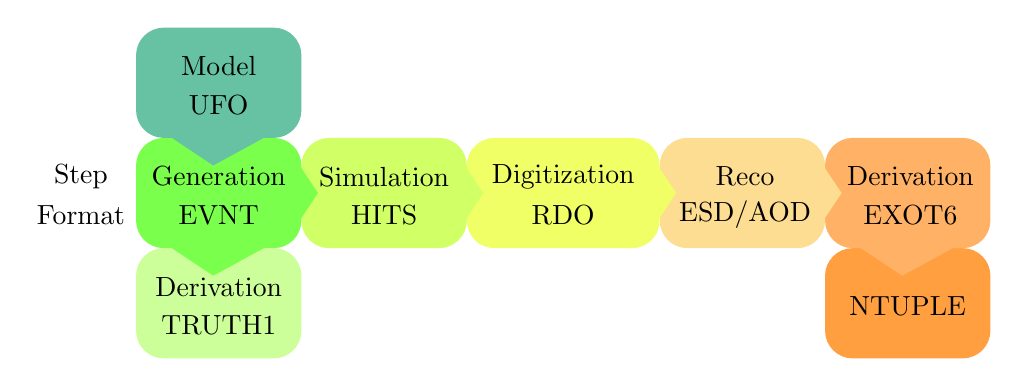
\begin{tikzpicture}[scale=0.7]

	\node[] at (-1,1.3){Step};
 	\node[] at (-1,0.6){Format};
 	
 	\draw[draw=none,fill=orange!75!, rounded corners=10pt] (12.5,0) rectangle +(3,-2);
 	\node[] at (1.5+12.5,-2+0.6+.35){NTUPLE};
 	
	\draw[draw=none,fill=orange!60!, rounded corners=10pt] (12.5,0) rectangle +(3,2);
 	\draw[draw=none,fill=orange!60!] (13,0.1)--(1.4+12.5,-0.5)--(2.5+12.5,0.1) -- cycle;
 	\node[] at (7.75+6.3,1.3){Derivation};
 	\node[] at (7.75+6.3,0.6){EXOT6};
	
	\draw[draw=none,fill=yellow!40!orange!40,rounded corners=10pt] (9.5,0) rectangle +(3,2);
 	\draw[draw=none,fill=yellow!40!orange!40] (12.4,0.4)--(12.8,1)--(12.4,1.6) -- cycle;
 	\node[] at (7.75+3.3,1.3){Reco};
 	\node[] at (7.75+3.3,0.6){ESD/AOD};
	
	\draw[draw=none,fill=green!10!yellow!60,rounded corners=10pt] (6,0) rectangle +(3.5,2);
 	\draw[draw=none,fill=green!10!yellow!60] (9.4,0.4)--(9.8,1)--(9.4,1.6) -- cycle;
 	\node[] at (7.75,1.3){Digitization};
 	\node[] at (7.75,0.6){RDO};
	
	\draw[draw=none,fill=green!30!yellow!60,rounded corners=10pt] (3,0) rectangle +(3,2);
 	\draw[draw=none,fill=green!30!yellow!60] (5.9,0.4)--(6.3,1)--(5.9,1.6) -- cycle;
 	\node[] at (4.5,1.3){Simulation};
 	\node[] at (4.5,0.6){HITS};
 	
 	\draw[draw=none,fill=green!75!yellow!70,rounded corners=10pt] (0,0) rectangle +(3,2);
	\draw[draw=none,fill=green!50!yellow!40,rounded corners=10pt] (0,0) rectangle +(3,-2);
 	\draw[draw=none,fill=green!75!yellow!70] (2.9,0.4)--(3.3,1)--(2.9,1.6) -- cycle;
 	\draw[draw=none,fill=green!75!yellow!70] (.5,0.1)--(1.4,-0.5)--(2.5,0.1) -- cycle;
 	
 	\node[] at (1.5,1.3){Generation};
 	\node[] at (1.5,0.6){EVNT};
 	\node[] at (1.5,-2+1.3){Derivation};
 	\node[] at (1.5,-2+0.6){TRUTH1};
 	
 	\draw[draw=none,fill=green!60!blue!60,rounded corners=10pt] (0,2) rectangle +(3,2);
 	\draw[draw=none,fill=green!60!blue!60] (.5,2.1)--(1.4,1.5)--(2.5,2.1) -- cycle;
 	\node[] at (1.5,3.3){Model};
 	\node[] at (1.5,2.6){UFO};
 	
 	%\node[] at (10.5,1.3){Reconstruction};
 	%\node[] at (10.5,0.6){ESD/AOD};

	%\node[ single arrow , draw, single arrow head extend=.7cm, gray!50, black] at (3.3,0.8) {    };
\end{tikzpicture}
}
\caption{The ATLAS simulation chain. The theoretical model is implemented in a UFO file and given as input to the generation program. Truth level analysis can be pursued, or the EVNT file can be used in a detector simulation whose outcome will be digitized in a RawData Object file and reconstructed in Event Summary Data (ESD) and Analysis Object Data (AOD). A derivation framework runs over the AOD to get the relevant events for a specific analysis. The Derivated Analysis Object Data (DAOD), which in our case is an EXOT6 file, can be made readable by RooT in a NTUPLE form.}
\label{fig:chain}
\end{figure}


\section{Generation}
 \begin{figure}[tp]
 \centering
 \begin{tikzpicture}
 [scale=0.5,decoration={
markings,% switch on markings
mark=% actually add a mark
at position .5  with {\arrow{>}}}]
 \draw[thick, postaction={decorate}] (-4,2) node at(-3,1)[above=2pt] {  $q$} -- (-2,0) ;
 \draw[thick, postaction={decorate}] (-2,0) -- (-4,-2) node at(-3,-1) [below=2pt] {  $\bar{q}$} ;
 \draw[thick,decorate,decoration={snake,amplitude=1.5mm,segment length=3.5mm}] (-2,0)--(1,0) node  at (-0.25,0) [below=3pt]{  $\gamma$,$\Zboson$};
 \draw[thick, postaction={decorate}] (1,0) -- (3,1) node at (2,0.5) [above]  {  $\chi^{\pm}$} ;
 \draw[thick, postaction={decorate}] (3,-1) --(1,0) node at (2,-0.5) [below=2pt]  {  $\chi^{\mp}$} ;
\draw[thick](3,1)--(3.4,2) node[above] {  $\pi^{\pm}$};
\draw[thick,postaction={decorate}](3,1)--(4.3,1.5) node[right=5pt,below] at (3.5,1.24) {  $\chi_0$};
\draw[thick](3,-1)--(3.4,-2) node[below] {  $\pimp$};
\draw[thick,postaction={decorate}](4.3,-1.5)--(3,-1) node[right=5pt,above] at (3.5,-1.24) {  $\chi_0$};
\draw[thick,decorate,decoration={snake,amplitude=1.5mm,segment length=8mm}] (-2.65,0.68)--(1,2) node at (-1,1.5) [above]{  $\gamma$};


 \draw[thick, postaction={decorate}] (-4+10,2) node at(-3+10,1)[above=2pt] {  $q$} -- (-2+10,0) ;
 \draw[thick, postaction={decorate}] (-2+10,0) -- (-4+10,-2) node at(-3+10,-1) [below=2pt] {  ${q'}$} ;
 \draw[thick,decorate,decoration={snake,amplitude=1.5mm,segment length=3.5mm}] (-2+10,0)--(1+10,0) node  at (-0.5+10,0) [below=3pt]{  $W^{\pm}$};
 \draw[thick, postaction={decorate}] (1+10,0) -- (3+10,1) node at (2+10,0.5) [above]  {  $\chi^{\pm}$} ;
 \draw[thick, postaction={decorate}] (3.6+10,-1.2) --(1+10,0) node at (1.8+10,-0.6) [below=12pt, right]  {  $\chi^{0}$} ;
\draw[thick](3+10,1)--(3.4+10,2) node[above] {  $\pi^{\pm}$};
\draw[thick,postaction={decorate}](3+10,1)--(4.3+10,1.5) node[right=5pt,below=1pt] at (3.5+10,1.24) {  $\chi_0$};

\draw[thick,decorate,decoration={snake,amplitude=1.5mm,segment length=7mm}] (0.07+10,0)--(1.8+10,-2.6) node at (0.9+10,-1.3) [below left=2pt]{  $\gamma$};

 \draw[thick, postaction={decorate}] (-4+5,2-6) node at(-3+5,1-6)[above=2pt] {  $q$} -- (-2+5,0-6) ;
 \draw[thick, postaction={decorate}] (-2+5,0-6) -- (-4+5,-2-6) node at(-3+5,-1-6) [below=2pt] {  ${q'}$} ;
 \draw[thick,decorate,decoration={snake,amplitude=1.5mm,segment length=3.5mm}] (-2+5,0-6)--(1+5,0-6) node  at (-0.5+5,0-6) [below=3pt]{  $W^{\pm}$};
 \draw[thick, postaction={decorate}] (1+5,0-6) -- (3+5,1-6) node at (2+5,0.5-6) [above]  {  $\chi^{\pm}$} ;
 \draw[thick, postaction={decorate}] (3.6+5,-1.2-6) --(1+5,0-6) node at (1.8+5,-0.6-6) [below=12pt, right]  {  $\chi^{0}$} ;
\draw[thick](3+5,1-6)--(3.4+5,2-6) node[above] {  $\pi^{\pm}$};
\draw[thick,postaction={decorate}](3+5,1-6)--(4.3+5,1.5-6) node[right=7pt,below] at (3.5+5,1.24-6) {  $\chi_0$};

\draw[thick,decorate,decoration={snake,amplitude=1.5mm,segment length=7.4mm}] (2+5,0.5-6)--(5.3+5,0.2-6) node at (3.65+5,0.35-6) [below=14pt,right=6pt]{ $\gamma$};
\end{tikzpicture}
\caption{Illustration of some Feynman diagrams for \mph processes in the Minimal DM Model.}
\label{fig:feynman}
\end{figure}
For the event generation process \MGMCatNLO v2.4.0 was used~\cite{madgraph}. This software automatically generates matrix elements, as for example decays or scattering from a couple of particles. The user simply specifies the process of interest by giving the initial and final state particles and \MADGRAPH generates the Feynman diagrams and the code needed for the calculation of the matrix elements~\cite{Pottgen:2016807}. In the context of the analysis, even if the software could generate matrix element up to the next to leading order (\NLO) only leading order (\LO) calculations were used.

The Minimal DM Model was already been implemented in an UFO file containing its details~\cite{mperego} considering the pure electroweak triplet (\chip\!, \chizero\!, \chim\!) and implemented in FeynRules. UFO is the format used in input by \MADGRAPH. Although the model would predict a mass splitting of \SI{\sim 165}{\mev} between \chipm and the \chizero, here is set to be \SI{1}{\gev}: small enough to let the charged $\chi$s decay into soft pions and a \chizero but large enough not to create issues in the generation program. 

Events of the type: 
\begin{gather*}
p p \rarrow \chi^+ \chi^- \gamma,\, \chi^+ \rarrow \piplus \chi_0,\, \chi^- \rarrow \piminus \chi_0\\
p p \rarrow \chi^+ \chi_0 \gamma,\, \chi^+ \rarrow \piplus \chi_0\\
p p \rarrow \chi^+ \chi_0 \gamma,\, \chi^- \rarrow \piminus \chi_0
\end{gather*}
have been generated to provide a final stare characterized by one photon and missing transverse momentum (\met). The Minimal DM model predicts several ways in which DM can be produced and revealed within a \mph analysis. Three examples of Feynman diagram are given in \Fig{\ref{fig:feynman}}. Notice that a photon can also be radiated from the final state which is a peculiarity with respect to other DM simplified models adopted at LHC.

For 21 different $\chi_0$ masses, \num{10000} events have been generated requiring a kinematic cut on photon energy to be greater than \SI{130}{\gev} in order to populate the \mph analysis \mbox{phase space}x.

Before performing the hadronization and parton shower, a fast scan for different mass point running \MADGRAPH \emph{on-the-fly} was made in order to get an order of magnitude the values of the cross sections. Results are reported in \Tab{\ref{tab:xsectheo}}.

\begin{table}[pt]
\centering
\begin{tabular}{ccc}
\toprule
Mass[GeV]&Cross section [pb]&Error [pb]\\
\midrule
\num{1}& \num{0.3069}& \num{0.0020}\\
\num{10}& \num{0.2924}& \num{0.0020}\\
\num{50}& \num{0.01571}& \num{0.00013}\\
\num{100}& \num{4.67e-03 }& \num{0.03e-03}\\
\num{200}& \num{1.164e-03}& \num{0.009e-03}\\
\num{500}& \num{7.54e-05}&\num{0.05e-05}\\
\num{750}& \num{1.369e-05}& \num{0.009e-05}\\
\num{1000}& \num{3.169e-06}& \num{0.021e-06}\\
\bottomrule
\end{tabular}
\caption{Table listing the cross section expected from theory, for several mass points, taken from the \MADGRAPH \emph{on-the-fly} running.}
\label{tab:xsectheo}
\end{table}

For the parton showers, underlying event and hadronization, the output of \MADGRAPH has to be passed to an external program, which in our case is \PYTHIA v8.210~\cite{pythia}. This framework accounts for the generation, starting from a \emph{Les Houches Event} (LHE) file, of parton shower and underlying event, i.e. it creates colorless states from free quarks and gluons. \PYTHIA was set up with NNPDF23LO PDF and the A14 tuning. The output file produced is an EVNT file which can be used as input either for the detector simulation step or to produce a TRUTH file.

\subsection{Truth level validation}
\label{sec:truth}
The generation of the events as it were ``in vacuum'' is called \emph{Truth level}. Here no assumptions are made on the detector, but we only want to analyze the process and its outcome. The TRUTH1 is a file format coming from a Derivation framework, which will be better explained in \Sect{\ref{sec:derivation}}, and it contains all needed information at particle level.

A ``fiducial region'' can be defined to allow the re-interpretation of the data analysis results in terms of new physics models, like the Minimal DM model, providing useful constraints.
 
The pre-selection for \mph analysis, (\Sect{\ref{sec:SRselection}}), involves:
\begin{itemize}
\item photons with $\pt^\gamma>\SI{10}{\GeV}$ with $\abs{\eta_\gamma}<2.37$ and $1.37<\abs{\eta_\gamma}<1.52$;
\item electrons with $\pt^e>\SI{7}{\gev}$ with $\abs{\eta_e}<2.47$;
\item muons with $\pt^\mu>\SI{6}{\gev}$ with $\abs{\eta_\mu}<2.5$;
\item jets with $\ptjet>\SI{30}{\gev}$ with $\abs{\eta_{\textup{jet}}}<4.5$ not overlapping with electron or photon by $\DeltaR > 0.4$;
\end{itemize}
while the actual selection requires:
\begin{itemize}
\item $\met>\SI{150}{\gev}$;
\item leading photon with $\pt^\gamma > \SI{150}{\GeV}$;
\item \met significance: $\met/\sqrt{\sumET} > \SI{8.5}{\GeV^{1/2}}$;
\item no electrons nor muons and $N_\textup{jets}\le 1$ with $\Delta\phi_\textup{jet-\met}<0.4$ if any.
\end{itemize}

The validation of the TRUTH files produced for several \chizero masses consists in the check of the distribution of the main kinematic variables involved in the analysis. The results are shown in validation plots in \Fig{\ref{fig:validation}} after the preselection provided above, for different DM masses. Notice that the peak for low-$\pt^\gamma$ in \Fig{\ref{subfig:phpt}} rises because the leading photon could enter the crack region (\etaRange{1.37}{1.52}), for instance, and therefore doesn't pass the $\eta$ cuts, then a sub-leading photon is selected with lower momentum.
%\footnote{A weird behaviour has been noticed in \PYTHIA for which sometimes the leading photon converts in a couple $e^+e^-$ for apparently no reasons. These events, however, contribute to the sharp low peak but they occur in the 5\% of the case and they can be neglected}. 
Detailed analyisis on these events in terms of fiducial cross section will be given in \Sect{\ref{sec:fid}}.

\begin{figure}[t]
\centering
\subfloat[][Photon momentum for different masses. \label{subfig:phpt}]
{\includegraphics[width=.45\textwidth]{MCSample/canPhPtoverlap}} \quad
\subfloat[][Missing transverse momentum for different masses]
{\includegraphics[width=.45\textwidth]{MCSample/canMEToverlap}} \quad
\subfloat[][Pseudorapidity of the photon for different masses]
{\includegraphics[width=.45\textwidth]{MCSample/canEtaoverlap}} \quad
\subfloat[][Number of jets for different masses]
{\includegraphics[width=.45\textwidth]{MCSample/canNjetsoverlap}} \quad
\caption{Validation plots for the Minimal DM model. From these plots the evolution of the main kinematics variables can be seen as a function of DM mass. These plots are generated after the pre-selection cuts given in \Sect{\ref{sec:truth}}}
\label{fig:validation}
\end{figure}

\section{Simulation}
The standard simulation of ATLAS relies on the \geant particle simulation toolkit to simulate the interaction of particles with matter. This step takes as input the EVNT file from \PYTHIA, or any of the generators such \HERWIG and \SHERPA, and it is the most time expensive stage in the full simulation. The output is stored into an HITS file. To save time the framework allows the user to skip a certain number of events at the beginning of an input file by submitting $n$ jobs with $N$ events each to a $n\times N$ event input file and merged together at the end of the process.

%First of all comes the simulation initialization which is divided in three steps. Stage one of the initialization occurs as soon as Athena is started which is set to AtlasProduction 19.2.4.9. release. Here job properties provided by the user are locked, metadata that will be stored with the hit output file are gathered and the HIT file initialized. Finally service is created to interface with \geant which is not fully initialized at this stage. In stage two detector, physics regions, range cuts are created. Each piece of the ATLAS detector is constructed in GeoModel according to the geometry chosen, which in this work is \verb!ATLAS-R2-2015-03-01-00_VALIDATION!, and translated into an equivalent \geant geometry. Next, the Monte Carlo truth strategies, which are \verb!MC12! in this context, are added to the simulation.Then the magnetic field is loaded and every user action, which allows a user to insert pieces of code in various places throughout the simulation event loop, provided from the configuration command are initialized. The physics list (see below) used for simulation is also set at this point. The third stage completes the job preparation. assigning fast simulation models and runs \geant  software.

%A physics list contains all numerical models that describe the particles' interactions in the \geant simulation. The \geant Collaboration provides several combinations of these models for every possible physical outline. We used the \verb!FTFP_BERT! phisics list which is the current \geant default. Any further information can be found in~\cite{ftfpbert}.

To speed up the full simulation process a fast simulation approach can be adopted. In this work ATLFAST-II was used, which provides large statistics to supplement full simulation studies. It is made up from two components: the Fast ATLAS Tracking Simulation (Fatras) for the inner detector and muon system simulation and the Fast Calorimeter Simulation (FastCaloSim) for the calorimeter simulation~\cite{simulation}. 

In Fatras the geometry of the detector consists in a simplified description of the full detector geometry, which maintains the same descriptive accuracy for its sensitive parts, and all other detector components are approximated as simplified layers that carry a high-granularity density providing an improvement in CPU time by a factor \num{100}. The interactions of the particles with the simplified detector layers are simulated using several methods, for instance ionization and radiative energy loss are simulated according to the Bethe-Bloch model. The photon conversion into a couple of electron and positron is performed depending on the thickness of the material crossed and hadronic interactions with the detector layer are simulated from parametric models obtained from \geant simulation results. Fatras provides also the input particle collection to give to FastCaloSim. Moreover it records energy deposition for muons in the calorimeter layers which will be used in the FastCaloSim application. The trajectories of the muons are also simulated in the muon spectrometer.

FastCaloSim uses parametrization of the longitudinal and lateral energy profile of the energy of single particle showers instead of simulating the particle interactions with the detector material. The parametrization are based on a fully-simulated, with \textsc{Geant4}, sample of 30 million events made of single photons and charged pions from an energy range between \SI{200}{\MeV} and \SI{500}{\GeV} for \AetaRange{5.0}. Electron and photon showers are approximated by the photon parametrization and hadronic showers are modeled on the charged pions.

The output from this simulation is a HITS file. The hits are records of energy deposition, with position and time, during the simulation. Most of them comes from the Inner Detector for which the majority of hits are independently stored and occupying about \SI{1360}{kB} per event while the muon system collects far fewer hits than the other subsystems and requires less disk space for the hit records (\SI{\sim3}{kB\per event}).

In order to understand anomalies and debug errors due to geometry or checking by eye overlaps and touching volumes in geometry a visualization step could also be performed. An examples of events are shown in \Fig{\ref{fig:simulation}}.

\begin{figure}[tp]
\centering
\includegraphics[width=.75\textwidth]{MCSample/simulation}
\caption{An event display made with VP1. VP1 is a viewing software made specifically for ATLAS which stands for Virtual Point 1, since ATLAS is situated at Point 1 of the LHC ring. It shows a Higgs boson decaying into four muons (shown in red). Inner detector tracks are in green, and energy deposited in the calorimeter by the muons is shown in yellow.}
\label{fig:simulation}
\end{figure}

\section{Digitization}
The ATLAS digitization software converts the hits produced by the core simulation into detector responses i.e ``digits''. In real events a digit is produced when a signal is recorded in a readout channel of the detector~\cite{simulation}.

In addition to the hard scattering digitization, \pileup and any other source of noise must be incorporated. For pile-up simulation, there are also input HITS files for minimum bias events to be overlaid, whose number for each bunch crossing is a function of the luminosity simulated. Moreover cavern background and cosmic muons could influence the simulation and they must be taken into account.
The ATLAS detector electronic produces data in byte-stream format called Raw Data Objects (RDO) whose size on disk is typically \SI{2.5}{MB\per event} and increases with larger number of \pileup events.

\section{Reconstruction}
\label{sec:recoreal}

Within this section, physics object definition and reconstruction in ATLAS are discussed, focusing on those mainly involved in this analysis. Definitions follow the recommendations from the various Combined Performance (CP) groups.

A reconstructed event in ATLAS is an ensemble of signals produced in the detector, which must be processed in order to get each particle property and identification. 

This step is identical for both real data and MC generated events and produces an output file in a Event Summary Data (ESD) and Analysis Object Data (AOD) form. 

\subsection{Photons}
\label{photons}
\subsubsection{Reconstruction}
Photons are reconstructed from clusters in the electromagnetic calorimeter measured in projective towers, even f the reconstruction uses information also from the Inner Detector. These towers are portions of the second layer of the calorimeter of $N_1 \times N_2$ cells in the $\eta-\phi$ plane. Photons and electrons (positrons) signature and energy deposits are very similar in the EM calorimeter. That's why information from ID to discriminate them are essential: a photon would not produce any track since the ID is sensitive only to charged particles. A cluster with no tracks associated is classified as a \emph{unconverted} photon since it was produced in a primary vertex it is straight revealed by the EM calorimeter. A \emph{converted} photon, instead, is produced in a primary vertex, it generates a electron-positron pair in a secondary vertex, within the ID, whose tracks can be associated to the cluster.

The reconstruction process starts from a \emph{sliding-window} algorithm which looks for the optimal deposit clusters. It starts from windows of $3\times5$ cells, or $0.025\times0.025$ in $\eta-\phi$, for unconverted photons and $3\times7$ cells ($0.175\times0.175 \, \eta\times\phi$) for converted ones, in the barrel region of the EM calorimeter, whose energy deposited is greater than \SI{2.5}{\gev}. In the end-cap, clusters of size $5\times5$ are used for all photon candidates.

%In order to identify an object as a photon or electron, tracks information is necessary. The tracking algorithm, Gaussian Sum Filter (GSF), reconstructs tracks by fitting points within the pixel detector and first layers of SCT and extrapolates informations gathered to outer layer of the ID and into the EM calorimeter. The algorithm also carefully trests the energy losses due to bremsstrahlung. Working along with the tracking algorithm, the vertexing algorithm analyses and classifies the interaction vertices and requires that a track points toward the center of the cluster whithin a $0.05\times0.05$ $\eta\times\phi$ window. Clusters with no matching tracks are classified as unconverted photons. Otherwise it is reconstructed as a converted photon or an electron.

Any noisy or sporadic noisy channel can sometimes produce a signal with transverse momentum larger than \SI{2.5}{\GeV} and give rise to a sliding window cluster~\cite{photons}. In order to identify these bad quality or fake clusters coming from instrumental problems cleaning cuts are applied on photon candidates. 

\subsubsection{Identification}
\begin{figure}[tp]
\centering
\includegraphics[width=.65\textwidth]{MCSample/pizerogamma}
\caption{Discrimination between a single photon and two collimated photons from a \pizero decay in the the ATLAS EM calorimeter. From the bottom to the top the strip, middle and back layers are visualized.}
\label{pizerogamma}
\end{figure}

Once a list of candidate photons has been made, we have to discriminate between real photons and hadronic jets containing high \pt \pizero, as shown in \Fig{\ref{pizerogamma}}. Identification is based upon the information from the strip and middle layers of the EM calorimeter.

Two working points are defined for photons: loose and tight depending on which cuts a photon passes based on shower shapes measured in strips and middle layers of the EM calorimeter together with hadronic leakage. The differences observed between data and MC in the discriminating variables are measured comparing the shower shape distributions in data and MC, parametrized as simple shifts. Instead, three working points which are loose, medium and tight, are defined for electrons. Details on photons selection criteria can be found in \cite[Sect. 4]{photons}.

Identification efficiency is computed with three different data-driven methods presented in~\cite{photons}: the matrix method, the electron extrapolation and the measurement of radiative photons from \mbox{\Zboson\rarrow\ellell$\gamma$} decays. Their efficiency comparison is given in \Fig{\ref{fig:phID}} for unconverted photons. Tight photons efficiency identification is expected to be greater than \SI{90}{\percent}.

\begin{figure}[pt]
\centering
\includegraphics[width=0.65\textwidth]{MCSample/phID}
\caption{Comparison of the data-driven measurements of the identification efficiency for unconverted photons as function of \et in the region \SIrange{10}{1500}{\gev}, for the pseudorapidity interval \AetaRange{0.6} using data collected in 2015-2016.}
\label{fig:phID}
\end{figure}

\subsubsection{Isolation}
\label{sec:phisolation}
\begin{figure}[tp]
\centering
\includegraphics[width=0.4\textwidth]{MCSample/topoetcone40}
\caption{The algorithm which fills TopoEtCone40 variable in action: from the $R=0.4$ cone (yellow) a $5\times7$ rectangle is removed, energy deposited is computed among the \topo~(orange) within the cone and the \pt-leakage (blue) is subtracted.}
\label{topoetcone40}
\end{figure}

Usually the isolation of a particle is expressed in terms of the $E_\textup{T}^{\textup{iso}}$ variable, which computes the transverse energy measured in the calorimeter cells (\topo) within a cone of given radius around the candidate. A track isolation $p_\textup{T}^{\textup{iso}}$variable can be defined as well.

In the above mentioned cone, an algorithm sums up the energies of the \topo~with energy deposits above a certain threshold~\cite{photonsISO}. The contribution of the photon itself, in a $5\times7$ cells area around the cone axis, and from the underlying evens and \pileup is  subtracted and the \pt-leakage, i.e. photon energy escaped from the area previously identified, is taken into account. Then the total energy in the cone is computed and the variable storing this information in this analysis is ``TopoEtCone40'' which contains the energy evaluated in a cone of radius $R=0.4$. Therefore a photon is considered isolated if ``TopoEtCone40''remains below a certain threshold, i.e. $\text{TopoEtcone40} < 0.022\pt^\gamma + \SI{2.45}{\GeV}$ and $\text{ptcone20}/\pt^\gamma<0.05$. A visual representation of the process described is given in \Fig{\ref{topoetcone40}}.

Isolation efficiency is computed to be greater than \SI{90}{\percent} for $\et^\gamma$ greater than \SI{100}{\gev}~\cite{photonsISO}.

\subsection{Missing transverse momentum}
\label{sec:met}
\subsubsection{Reconstruction}

An intuitive definition of missing transverse momentum (\met) is the momentum inbalance in the transverse plane. A non-zero inbalance, must suggest the presence of missing energy since this plane is boost-invariant and energy must be conserved. Indeed we can state something only about transverse energy since the parton momentum in the beam direction before the collision is unknown.

The true \met is given simply by neutrinos and non interacting particles, but there are also other sources, such malfunctioning detector region or its finite coverage, that creates fake \met due to a bad or missing reconstruction of physics objects. This is particularly relevant for this analysis when we look for \emph{non}-interacting particles such DM particles.

The \met calculation used in this analysis is based on all reconstructed and calibrated physics objects. In the transverse plane the \met magnitude and the corresponding azimuthal angle are given by:
\begin{gather}
\label{eqn:met}
	\met=\sqrt{(E_x^\textup{miss})^2+(E_y^\textup{miss})^2}\\
	\phi^\textup{miss}=\arctan\big({E_y^\textup{miss}/E_x^\textup{miss}}\big)
\end{gather}

The single components $E_i^\textup{miss}$, ($i=\{x,y\}$), in equation \ref{eqn:met} is given by:
\begin{equation}
	E_i^\textup{miss}=E_i^\textup{miss,$e$}+E_i^\textup{miss,$\gamma$}+E_i^\textup{miss,$\mu$}+E_i^\textup{miss,$\tau$}+E_i^\textup{miss,jets}+E_i^\textup{miss,Soft}
\end{equation}

Each term is calculated as the negative sum of the momentum of the reconstructed objects projected onto the $x$ and $y$ direction of the transverse plane. The ``Soft'' term is calculated from energy deposits or tracks which are not matched to selected hard objects. 

There are several computation of \met, as explained in~\cite{met}. The one this analysis is based on is the ``Track Soft Term'' (TST) as recommended by ATLAS Jet/Etmiss Combined Performance groups, calculated from the tracks from the primary vertices that are not matched to selected hard objects and providing a stronger measurement against \pileup~\cite{met}.

\section{EXOT6 Derivation}
\label{sec:derivation}
During the \RunTwo ATLAS has developed a ``Derivation Framework'', by proposal by the Analysis Model Study Group (AMSG), which works on the principle that analyzers need to be able to run over their data sample frequently. For this purpose the derivation framework provides the offline software tools and structures to work on data in a very simple way~\cite{twiki:DAOD}. 

Unlike in \RunOne, when derivation was made by users, this production is now made centrally by the ATLAS production services, even if it can be run locally as in our case, avoiding difficulties in cross-team analyses due to differences in the formats and in reading the output file.

Derivations are made from the reconstructed data via four operations:
\begin{enumerate}
\item skimming: the removal of entire events;
\item thinning: when removing the whole object in an event, but keeping the rest of it;
%(for instance an electron is totally removed while other object remains),
\item slimming: information removal from objects, while keeping the rest of it; 
%(i.e. only certain object information ,such its transverse momentum. are removed but the object still remains in the event),
\item augmentation: adding informations not found in the input data.
\end{enumerate}

Therefore the derivation framework selects only the relevant data for a specific analysis, from all ATLAS data collected. This functioning is well explained in the sketch shown in \Fig{\ref{fig:derivation}}.

For this analysis a specific derivation called ``EXOT6'' has been implemented and the following skimming selection was applied:
\begin{itemize}
\item Events must pass one out of several trigger request, including the \verb!HLT_g140_loose! which this analysis is based on;
\item Events must have one loose
%\footnote{see \Sect{\ref{photons}}} 
photon with $\pt\ge\SI{80}{\gev}$ or one loose electron with \mbox{$\pt\ge\SI{100}{\gev}$}.
\end{itemize}

As final step a ROOT::NTUPLE file was produced in which events are selected following the recommendation by the Combined Performance groups. The analysis code is based on SUSYTools-00-08-20 based on AnalysisBase 2.4.28. Details on object definition and kinematic cuts performed in the SUSYTools code are given in~\cite{twiki:SUSYTools}.


\begin{figure}[tb]
\centering
\includegraphics[width=.48\textwidth]{MCSample/Derivation}
\caption{Sketch of how the derivation code works for ATLAS data. Each single event from the whole amount of dara contains different characteristics that the derivation code depending on the analysis performed.}
\label{fig:derivation}
\end{figure}

















\backmatter
\appendix
\chapter{Systematic Table}
\lipsum

\newgeometry{left=0.1cm,right=0.1cm}

\begin{longtable}{lccccc}

  \noalign{\footnotesize} 
  \toprule 
  Systematic & SR & ONEmuCR & TWOmuCR & TWOeleCR & PhJetCR \\
  \midrule
  \endfirsthead
  
  \multicolumn{6}{l}{\footnotesize\itshape Continua dalla pagina precedente} \\
  \toprule
  Systematic & SR & ONEmuCR & TWOmuCR & TWOeleCR & PhJetCR \\
  \midrule
  \endhead
  
  \midrule
  \multicolumn{6}{l}{\footnotesize\itshape Continua nella pagina precedente} \\
  \endfoot
  
  \bottomrule
  \multicolumn{6}{l}{\footnotesize\itshape Si conlcude dalla pagina precedente} \\
  \endlastfoot

  alpha\_EG\_RESO & ($-0.00$, $0.06$) & ($-0.00$, $0.00$) & ($0.09$, $-0.04$) & ($-0.10$, $0.05$) & ($-0.00$, $-0.01$) \\ \noalign{\smallskip} 
  alpha\_EG\_SCALE & ($0.16$, $-0.13$) & ($-0.00$, $0.00$) & ($0.09$, $-0.06$) & ($-0.12$, $0.10$) & ($-0.00$, $-0.00$) \\ \noalign{\smallskip} 
  alpha\_EL\_EFF\_ID & ($-0.75$, $0.81$) & ($0.00$, $-0.02$) & ($-1.09$, $1.11$) & ($1.38$, $-1.40$) & ($-0.00$, $0.00$) \\ \noalign{\smallskip} 
  alpha\_EL\_EFF\_ISO & ($-0.36$, $0.40$) & ($-0.00$, $-0.00$) & ($-0.53$, $0.53$) & ($0.68$, $-0.69$) & ($-0.00$, $0.00$) \\ \noalign{\smallskip} 
  alpha\_EL\_EFF\_RECO & ($-0.30$, $0.30$) & ($0.00$, $-0.00$) & ($-0.39$, $0.40$) & ($0.52$, $-0.52$) & ($-0.00$, $0.00$) \\ \noalign{\smallskip} 
  alpha\_EleFake\_statCR\_ONEmuCR & ($-0.02$, $0.02$) & ($0.01$, $-0.01$) & ($-0.01$, $0.02$) & ($-0.01$, $0.01$) & ($-0.00$, $-0.00$) \\ \noalign{\smallskip} 
  alpha\_EleFake\_statCR\_PhJetCR & ($-0.00$, $0.00$) & ($-0.00$, $0.00$) & ($-0.00$, $0.00$) & ($-0.00$, $0.00$) & ($-0.00$, $-0.00$) \\ \noalign{\smallskip} 
  alpha\_EleFake\_statCR\_SR & ($0.07$, $-0.07$) & ($0.00$, $0.00$) & ($0.00$, $0.00$) & ($0.00$, $0.00$) & ($0.00$, $0.00$) \\ \noalign{\smallskip} 
  alpha\_EleFake\_statCR\_TWOeleCR & ($-0.00$, $0.00$) & ($-0.00$, $0.00$) & ($-0.00$, $0.00$) & ($0.02$, $-0.02$) & ($0.00$, $0.00$) \\ \noalign{\smallskip} 
  alpha\_EleFake\_statCR\_TWOmuCR & ($-0.00$, $0.01$) & ($-0.00$, $0.00$) & ($0.03$, $-0.02$) & ($-0.00$, $0.02$) & ($0.00$, $-0.00$) \\ \noalign{\smallskip} 
  alpha\_EleFake\_stat\_ONEmuCR & ($-0.03$, $0.02$) & ($0.01$, $-0.01$) & ($0.00$, $-0.01$) & ($0.02$, $-0.02$) & ($-0.00$, $-0.00$) \\ \noalign{\smallskip} 
  alpha\_EleFake\_stat\_PhJetCR & ($-0.00$, $0.00$) & ($0.00$, $-0.00$) & ($0.00$, $-0.00$) & ($0.00$, $0.00$) & ($0.00$, $-0.00$) \\ \noalign{\smallskip} 
  alpha\_EleFake\_stat\_SR & ($0.68$, $-0.68$) & ($0.00$, $0.00$) & ($0.00$, $0.00$) & ($0.00$, $0.00$) & ($0.00$, $0.00$) \\ \noalign{\smallskip} 
  alpha\_EleFake\_stat\_TWOeleCR & ($-0.00$, $0.00$) & ($-0.00$, $0.00$) & ($-0.00$, $0.00$) & ($0.00$, $-0.00$) & ($-0.00$, $0.00$) \\ \noalign{\smallskip} 
  alpha\_EleFake\_stat\_TWOmuCR & ($-0.00$, $0.00$) & ($-0.00$, $0.00$) & ($0.02$, $-0.02$) & ($-0.00$, $0.00$) & ($0.00$, $0.00$) \\ \noalign{\smallskip} 
  alpha\_EleFake\_syst\_ONEmuCR & ($-0.07$, $0.07$) & ($0.00$, $-0.01$) & ($0.01$, $-0.00$) & ($0.01$, $-0.00$) & ($-0.00$, $-0.00$) \\ \noalign{\smallskip} 
  alpha\_EleFake\_syst\_PhJetCR & ($-0.01$, $0.04$) & ($-0.00$, $-0.00$) & ($0.01$, $0.00$) & ($0.00$, $-0.00$) & ($0.00$, $-0.00$) \\ \noalign{\smallskip} 
  alpha\_EleFake\_syst\_SR & ($1.34$, $-1.34$) & ($0.00$, $0.00$) & ($0.00$, $0.00$) & ($0.00$, $0.00$) & ($0.00$, $0.00$) \\ \noalign{\smallskip} 
  alpha\_EleFake\_syst\_TWOeleCR & ($-0.00$, $0.00$) & ($-0.00$, $0.00$) & ($-0.00$, $0.00$) & ($0.01$, $-0.01$) & ($-0.00$, $0.00$) \\ \noalign{\smallskip} 
  alpha\_EleFake\_syst\_TWOmuCR & ($-0.00$, $0.01$) & ($-0.00$, $0.00$) & ($0.03$, $-0.02$) & ($-0.00$, $0.02$) & ($0.00$, $-0.00$) \\ \noalign{\smallskip} 
  alpha\_JER & ($-0.56$, $0.67$) & ($-0.00$, $-0.00$) & ($-0.11$, $0.10$) & ($0.15$, $-0.15$) & ($0.00$, $0.00$) \\ \noalign{\smallskip} 
  alpha\_JES & ($-4.09$, $1.78$) & ($-0.00$, $-0.00$) & ($-0.28$, $0.14$) & ($0.36$, $-0.17$) & ($-0.00$, $-0.00$) \\ \noalign{\smallskip} 
  alpha\_JVT\_EFF & ($-0.01$, $0.04$) & ($-0.00$, $0.01$) & ($-0.01$, $0.00$) & ($0.01$, $-0.02$) & ($-0.00$, $0.00$) \\ \noalign{\smallskip} 
  alpha\_JetFake\_statCR\_ONEmuCR & ($-0.27$, $0.22$) & ($0.00$, $-0.00$) & ($-0.02$, $-0.03$) & ($0.01$, $-0.02$) & ($-0.00$, $-0.00$) \\ \noalign{\smallskip} 
  alpha\_JetFake\_statCR\_PhJetCR & ($-0.03$, $0.06$) & ($0.00$, $-0.00$) & ($-0.00$, $0.00$) & ($-0.02$, $-0.00$) & ($0.00$, $-0.00$) \\ \noalign{\smallskip} 
  alpha\_JetFake\_statCR\_SR & ($0.81$, $-0.81$) & ($0.00$, $0.00$) & ($0.00$, $0.00$) & ($0.00$, $0.00$) & ($0.00$, $0.00$) \\ \noalign{\smallskip} 
  alpha\_JetFake\_statCR\_TWOeleCR & ($-0.46$, $0.48$) & ($-0.00$, $0.00$) & ($-0.67$, $0.62$) & ($1.01$, $-0.96$) & ($-0.00$, $-0.00$) \\ \noalign{\smallskip} 
  alpha\_JetFake\_statCR\_TWOmuCR & ($-0.70$, $0.68$) & ($-0.00$, $-0.00$) & ($0.50$, $-0.48$) & ($-0.73$, $0.72$) & ($0.00$, $-0.00$) \\ \noalign{\smallskip} 
  alpha\_LUMI\_SYST & ($0.04$, $-0.02$) & ($-0.00$, $-0.00$) & ($-0.01$, $-0.01$) & ($-0.03$, $-0.01$) & ($0.01$, $0.00$) \\ \noalign{\smallskip} 
  alpha\_MET\_RESO\_PARA & ($0.18$, $-0.10$) & ($-0.00$, $-0.00$) & ($0.02$, $-0.02$) & ($-0.03$, $0.02$) & ($-0.00$, $-0.01$) \\ \noalign{\smallskip} 
  alpha\_MET\_RESO\_PERP & ($0.24$, $-0.21$) & ($-0.00$, $0.01$) & ($-0.00$, $0.01$) & ($0.02$, $-0.02$) & ($-0.01$, $0.01$) \\ \noalign{\smallskip} 
  alpha\_MET\_SCALE & ($0.84$, $-0.79$) & ($0.01$, $-0.00$) & ($0.02$, $0.03$) & ($0.01$, $-0.04$) & ($-0.00$, $0.01$) \\ \noalign{\smallskip} 
  alpha\_MU\_EFF\_STAT & ($-0.13$, $0.33$) & ($-0.01$, $-0.01$) & ($0.04$, $-0.16$) & ($-0.05$, $0.17$) & ($-0.00$, $0.00$) \\ \noalign{\smallskip} 
  alpha\_MU\_EFF\_SYST & ($-0.81$, $1.00$) & ($-0.00$, $-0.00$) & ($0.52$, $-0.63$) & ($-0.67$, $0.78$) & ($-0.01$, $-0.00$) \\ \noalign{\smallskip} 
  alpha\_MU\_EFF\_SYST\_LOWPT & ($-0.08$, $0.28$) & ($-0.01$, $-0.01$) & ($0.02$, $-0.13$) & ($-0.01$, $0.14$) & ($-0.00$, $0.00$) \\ \noalign{\smallskip} 
  alpha\_MU\_ID & ($-0.10$, $0.20$) & ($0.00$, $-0.01$) & ($-0.01$, $-0.12$) & ($0.02$, $0.14$) & ($-0.00$, $-0.00$) \\ \noalign{\smallskip} 
  alpha\_MU\_ISO\_STAT & ($-0.13$, $0.33$) & ($-0.01$, $-0.01$) & ($0.04$, $-0.16$) & ($-0.04$, $0.17$) & ($-0.00$, $0.00$) \\ \noalign{\smallskip} 
  alpha\_MU\_ISO\_SYST & ($-0.37$, $0.60$) & ($0.00$, $-0.01$) & ($0.21$, $-0.31$) & ($-0.25$, $0.43$) & ($-0.00$, $0.00$) \\ \noalign{\smallskip} 
  alpha\_MU\_MS & ($-0.04$, $0.04$) & ($-0.01$, $-0.00$) & ($-0.01$, $-0.02$) & ($0.03$, $0.03$) & ($-0.00$, $-0.00$) \\ \noalign{\smallskip} 
  alpha\_MU\_SCALE & ($-0.01$, $0.08$) & ($-0.00$, $-0.00$) & ($-0.01$, $-0.11$) & ($0.02$, $0.13$) & ($-0.00$, $-0.00$) \\ \noalign{\smallskip} 
  alpha\_MU\_TTVA\_STAT & ($-0.07$, $0.27$) & ($-0.01$, $-0.01$) & ($0.01$, $-0.13$) & ($-0.00$, $0.13$) & ($-0.00$, $0.00$) \\ \noalign{\smallskip} 
  alpha\_MU\_TTVA\_SYS & ($-0.16$, $0.37$) & ($-0.01$, $-0.01$) & ($0.07$, $-0.19$) & ($-0.08$, $0.21$) & ($-0.00$, $0.00$) \\ \noalign{\smallskip} 
  alpha\_PDF\_Comb & ($0.06$, $-0.03$) & ($0.01$, $-0.00$) & ($0.01$, $-0.00$) & ($0.01$, $-0.00$) & ($0.00$, $-0.00$) \\ \noalign{\smallskip} 
  alpha\_PH\_EFF & ($-0.13$, $-0.00$) & ($0.01$, $-0.00$) & ($-0.03$, $-0.01$) & ($0.02$, $0.00$) & ($-0.01$, $-0.00$) \\ \noalign{\smallskip} 
  alpha\_PH\_EFF\_TRKISO & ($-0.01$, $0.04$) & ($-0.00$, $0.01$) & ($-0.01$, $0.00$) & ($0.01$, $-0.02$) & ($-0.00$, $0.00$) \\ \noalign{\smallskip} 
  alpha\_PH\_ISO\_DD & ($-0.01$, $0.04$) & ($-0.00$, $0.01$) & ($-0.01$, $0.00$) & ($0.01$, $-0.02$) & ($-0.00$, $0.00$) \\ \noalign{\smallskip} 
  alpha\_PRW\_DATASF & ($0.14$, $-1.31$) & ($-0.00$, $-0.00$) & ($-0.26$, $0.06$) & ($0.35$, $-0.07$) & ($0.00$, $-0.01$) \\ \noalign{\smallskip} 
  alpha\_syst\_JetFake\_ONEmuCR & ($-0.19$, $0.19$) & ($-0.00$, $-0.00$) & ($0.00$, $-0.02$) & ($-0.00$, $-0.02$) & ($-0.00$, $-0.00$) \\ \noalign{\smallskip} 
  alpha\_syst\_JetFake\_PhJetCR & ($-0.01$, $0.05$) & ($-0.00$, $-0.00$) & ($0.01$, $0.00$) & ($0.00$, $-0.00$) & ($0.00$, $-0.00$) \\ \noalign{\smallskip} 
  alpha\_syst\_JetFake\_SR & ($0.16$, $-0.16$) & ($0.00$, $0.00$) & ($0.00$, $0.00$) & ($0.00$, $0.00$) & ($0.00$, $0.00$) \\ \noalign{\smallskip} 
  alpha\_syst\_JetFake\_TWOeleCR & ($-0.30$, $0.31$) & ($-0.00$, $0.00$) & ($-0.38$, $0.41$) & ($0.62$, $-0.65$) & ($-0.00$, $-0.00$) \\ \noalign{\smallskip} 
  alpha\_syst\_JetFake\_TWOmuCR & ($-0.10$, $0.09$) & ($0.00$, $-0.01$) & ($0.08$, $-0.07$) & ($-0.11$, $0.11$) & ($-0.00$, $-0.00$) \\ \noalign{\smallskip} 
  alpha\_syst\_PhJet\_shape\_SR & ($-1.50$, $1.50$) & ($0.00$, $0.00$) & ($0.00$, $0.00$) & ($0.00$, $0.00$) & ($0.00$, $0.00$) \\ \noalign{\smallskip} 
  
\end{longtable}


\restoregeometry



\end{document}
